\section{\mpijm}

The MPI specification\cite{MPI} includes a mechanism by which a parent process can spawn a child process that receives its own \mpicommworld: \spawn.
After disconnecting the parent-child intercommunicator, the parent survives a child's \mpiabort, thereby making the parent robust against its children's problems.
It is around this structure \mpijm is built.

The \mpijm model consists of a master, a scheduler, and workers.
The master \jmmaster is launched on every node, and is responsible for launching and monitoring jobs, and reporting information to the scheduler.
The scheduler \jmscheduler is a single process that tracks the available resources, manages a queue of computational tasks, distributes those tasks to nodes, and collect status.
The workers are the user applications that will execute the computational work, linked against a library \jmworker.

\begin{figure}[t]
    \centering
        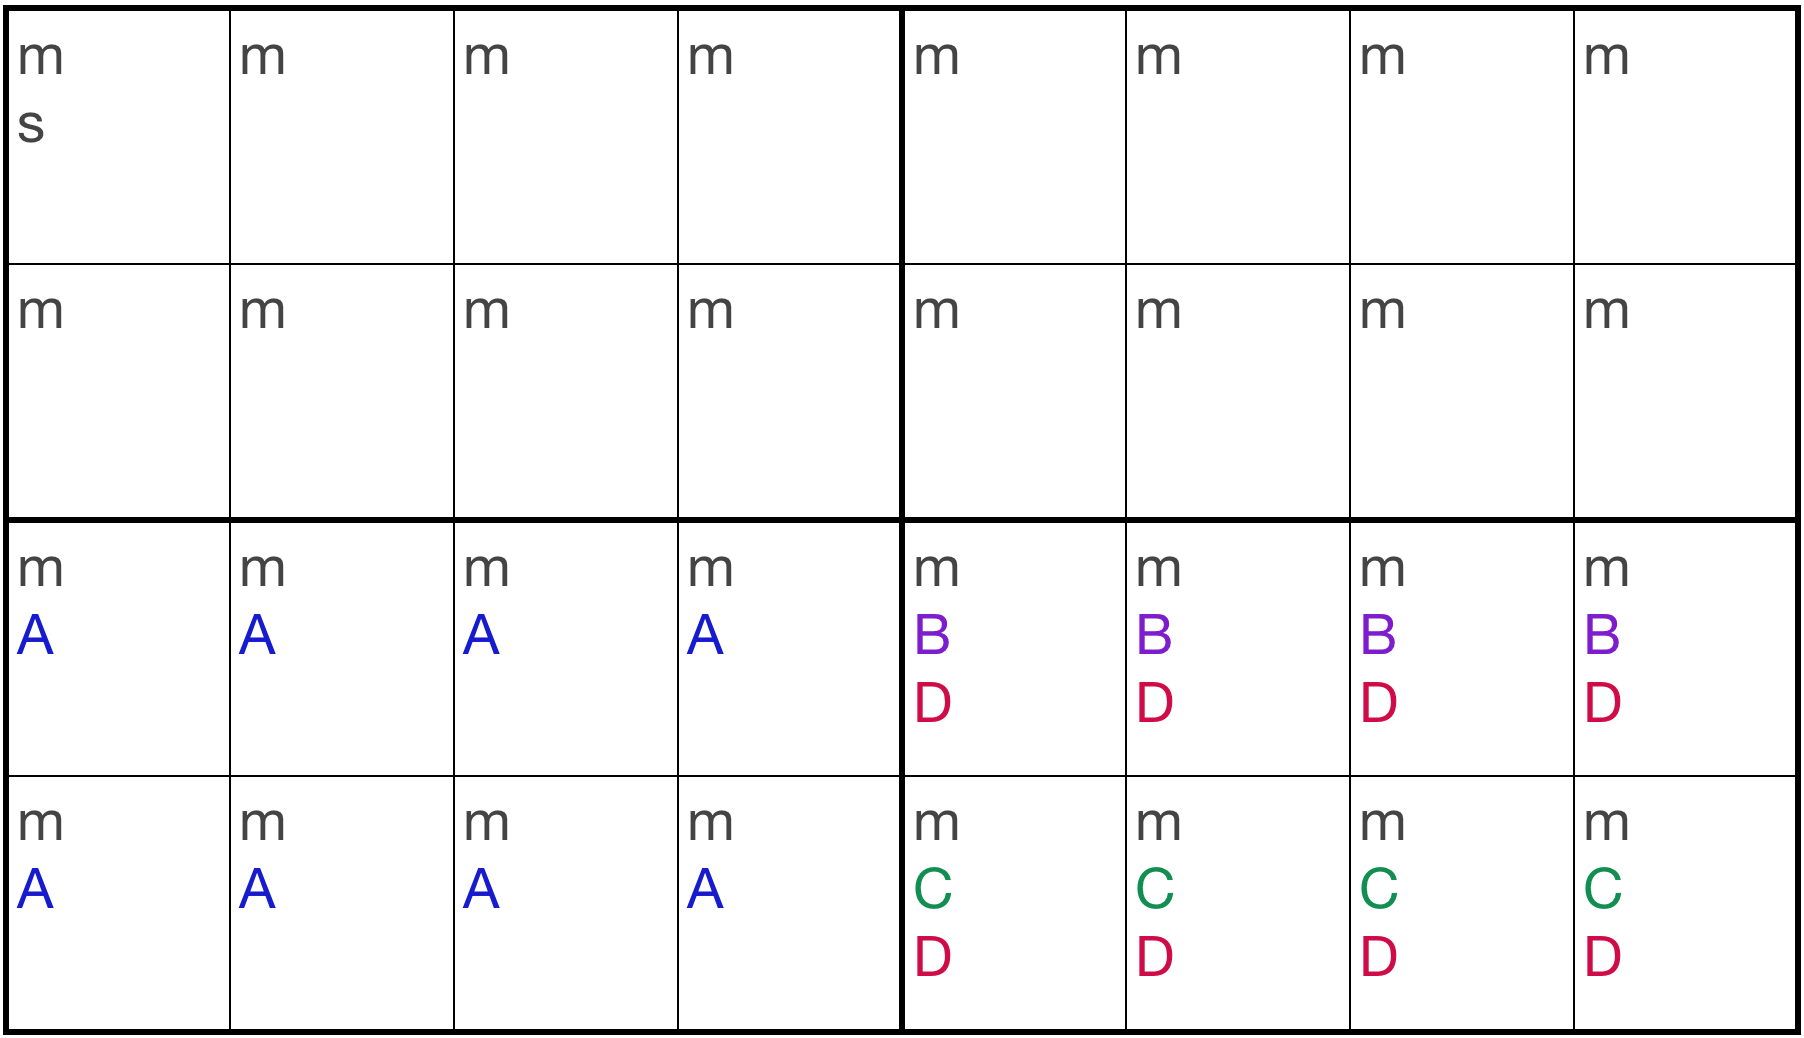
\includegraphics[width=\textwidth]{jm_example.png}
    \caption{An example 32-node layout, with four blocks of eight nodes.  Every node launches \jmmaster (m), one \jmscheduler (s) is spawned, and workers of different sizes (A, B, C, D) and requiring different resources are launched.  In this case, worker A consumes all the resources in a block, while B, C, and D can peacefully coexist in a block.  Perhaps D requires GPUs but only a few CPU cores, while B and C are CPU-intensive.}
    \label{fig:jm_example}
\end{figure}

\subsection{Masters}

\jmmaster is launched across the entire allocation with \mpirun (or equivalent), with one MPI task per node.
Each \jmmaster also reports its location in the system hierarchy, so that they may be organized into blocks with fast communication, avoiding resource fragmentation across the communication fabric.

\subsection{The Scheduler}

\subsection{Workers}

Workers require minimal modification.
After the \mpiinit of a user application, one adds a handshake \jmhandshake that reports to the local master and disconnects the communicator from the parent which launched it via \spawn.
One also adds \jmfinish just before \mpifinalize, allowing the worker to communicate its exit status and other information to its local master.

When workers are launched by the master via \spawn, they perform said handshake and reporting.
When workers are launched independently, they skip those steps, enabling the same binary to be launched in both ways.
This flexibility makes \mpijm-enabled applications easy to maintain, while also ensuring the same binary is executed during debugging as is executed during production.

\subsection{Dependencies}

